%% Los cap'itulos inician con \chapter{T'itulo}, estos aparecen numerados y
%% se incluyen en el 'indice general.
%%
%% Recuerda que aqu'i ya puedes escribir acentos como: 'a, 'e, 'i, etc.
%% La letra n con tilde es: 'n.




\chapter*{Introducci'on}
\addcontentsline{toc}{chapter}{Introducci'on}
\chaptermark{Introducci'on}

\section*{Antecedentes y Planteamiento del problema}
\addcontentsline{toc}{section}{Antecedentes y Planteamiento del problema}


El c'omputo en la nube es una tecnolog'ia que ha abarcado gran parte de los negocios  para dar soporte a ellos. 'Esta tecnolog'ia provee a los negocios una ventaja competitiva en los costos de recursos como se ve en los negocios tradicionales, adem'as de la versatilidad que provee al ajustarse a la necesidad de las empresas (\citeauthor{srinivasan2014cloud}, \citeyear{srinivasan2014cloud}).



%\cite{srinivasan2014cloud}. 

La tecnolog'ia en la nube ha desarrollado una infraestructura fuerte despu'es del surgimiento del c'omputo distribuido (\citeauthor{chen2009cloud}, \citeyear{chen2009cloud}). Para obtener las ventajas de dicha tecnolog'ia los usuarios simplemente necesitar'an conectarse a internet y de esta manera tendr'an el acceso al procesamiento de manera remota (\citeauthor{aranganathan2011aco}, \citeyear{aranganathan2011aco}). Sin embargo, para aprovechar el m'aximo potencial de 'estos recursos, es necesario tener en consideraci'on algunas variables, ya que en un entorno en la nube existe un comportamiento din'amico de los recursos a manera que se les provea a los usuarios el servicio (\citeauthor{shimpy2014different}, \citeyear{shimpy2014different}).
Una de las pr'acticas con mayor importancia en la nube es la calendarizaci'on, ya que tiene como objetivo administrar las tareas del centro de datos para optimizar los recursos del mismo. De esta manera la eficiencia de la carga de trabajo en la nube aumenta (\citeauthor{shimpy2014different}, \citeyear{shimpy2014different}).
En general, el objetivo de la calendarizaci'on en la nube es utilizar los recursos de manera apropiada, mientras la carga de trabajo es distribuida uniformemente para mejorar los tiempos de ejecuci'on (\citeauthor{shimpy2014different}, \citeyear{shimpy2014different}).
Debido a la atenci'on que se tiene en la tecnolog'ia en la nube, los centros de datos han tomado un papel muy importante para los servicios empresariales (\citeauthor{shimpy2014different}, \citeyear{shimpy2014different}). 
Un centro de datos est'a compuesto por miles de servidores virtuales ejecut'andose en una instancia de tiempo alojando muchas tareas, al mismo tiempo el centro de datos recibe miles de peticiones a esas tareas. Es aqu'i en donde la programaci'on de trabajos tiene un rol demasiado importante para el c'omputo en la nube, ya que influye en el rendimiento del mismo (\citeauthor{srinivasan2014cloud}, \citeyear{srinivasan2014cloud}). 

El problema de la calendarizaci'on pertenece a los algoritmos NP-Dif'icil, lo cual tiene un amplio rango de soluciones posibles y se toma mucho m'as tiempo de encontrar una respuesta ‘optima, ya que no existe un m'etodo para resolver estas inc'ognitas. Sin embargo, es posible estar cerca de la mejor soluci'on contemplando algunos entornos (\citeauthor{shimpy2014different}, \citeyear{shimpy2014different}).




\section*{Propuesta de soluci'on y Justificaci'on}
\addcontentsline{toc}{section}{Propuesta de soluci'on y Justificaci'on}


Los centros de datos son una parte esencial en la tecnolog'ia en la nube, est'an conformados por varios servidores virtuales que alojan varios trabajos, ejecut'andose por estancias de tiempo y a la vez recibiendo peticiones a esos trabajos (\citeauthor{shimpy2014different}, \citeyear{shimpy2014different}).
Para que el c'omputo en la nube pueda rendir correctamente, se necesita una buena programaci'on de trabajos o calendarizaci'on. Este problema tiene un gran n'umero de soluciones posibles, toma mucho tiempo en encontrar un respuesta 'optima y por eso est'a dentro de los algoritmos NP-Dif'icil. No existe un m'etodo para resolver lo anterior, sin embargo es posible obtener una soluci'on cercana comtemplando algunos entornos (\citeauthor{shimpy2014different}, \citeyear{shimpy2014different}).
En esta investigaci'on se propone una mejora a un algoritmo de calendarizaci'on para el caso de estudio de un sistema ERP en la nube, contemplando sus posibles escenarios y peticiones heterog'eneas. De esta manera se podr'a contar con un esquema de distribuci'on de trabajos que satisfaga las necesidades de un sistema ERP, mejorando el tiempo de respuesta y aprovechando los recursos. Con beneficios a los proveedores de servicios (SaaS) de sistemas ERP.

\newpage

\begin{figure}
	
	\centering
	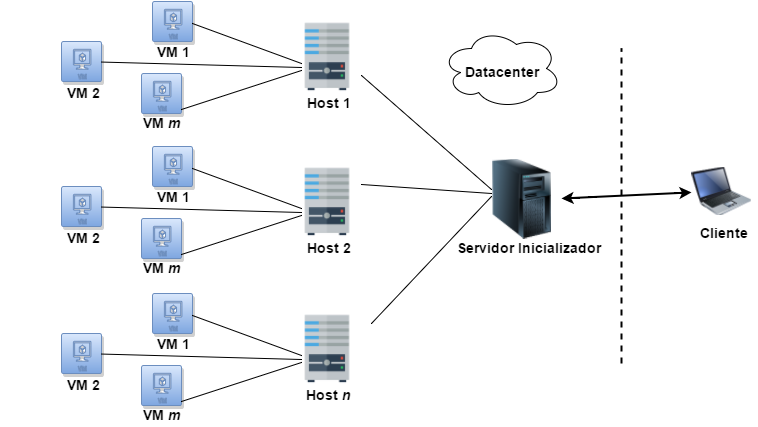
\includegraphics[scale=0.5]{media/cloud2}
	\caption{Propuesta de arquitectura en la nube, Fuente: Elaboraci'on propia. }
\end{figure}
%%%%%%%%
%%  IMAGEN
%%%


En la figura 1 se puede observar la arquitectura del centro de datos que se implementar'a en la investigaci'on, el cual est'a compuesto de los siguientes elementos:

\begin{itemize}
	\item \textbf{Servidor administrador:} Es el servidor que tendr'a el rol de front end en el centro de datos, teniendo una interacci'on directa con las peticiones de los usuarios, que son especificados en 'este documento como trabajos.
	El principal objetivo de 'este elemento es delegar los trabajos a las m'aquinas virtuales en los distintos hosts del centro de datos.
	\item \textbf{Host:} es el recurso de hardware que se tiene en el centro de datos. Una de las caracter'isticas de 'este elemento es que es finito.
	\item \textbf{M'aquinas Virtuales:} son instancias dentro de los host, tienen como objetivo resolver los trabajos que se les sea asignado.
\end{itemize}


\section*{Objetivos}
\addcontentsline{toc}{section}{Objetivos}


\subsection*{Objetivo general}
\addcontentsline{toc}{section}{Objetivo general}


Determinar y proponer un nuevo esquema que pueda resolver de manera eficiente el problema de la calendarizaci'on de un centro de datos y satisfacer las necesidades de un sistema ERP en la nube.


\subsection*{Objetivos espec'ificos}
\addcontentsline{toc}{section}{Objetivos espec'ificos}


\begin{itemize}
	\item Definir una arquitectura para un centro de datos en la nube con las necesidades de un sistema ERP.
	\item Realizar la simulaci'on en base a la arquitectura del centro de datos.
	\item Realizar e implementar diferentes esquemas de distribuci'on de trabajos, rescatando sus caracter'isticas principales.
	\item Reunir las caracter'isticas principales y proponer el nuevo esquema de distribuci'on.
	\item Aplicar el nuevo esquema de distribuci'on a las necesidades de un ERP.
	\item Comparar los resultados obtenidos del nuevo esquema propuesto y de los anteriores para determinar si hubo una mejora.
\end{itemize}


\newpage

\section*{Hip'otesis}
\addcontentsline{toc}{section}{Hip'otesis}

La modificaci'on de un esquema de distribuci'on mejorar'a el rendimiento de la calendarizaci'on para un sistema ERP en la nube.

Para realizar la verificaci'on de validez de la hip'otesis se usar'an:


\begin{itemize}
	\item \textbf{Pruebas de hardware y software:}
	\begin{itemize}
	\item \textbf{Prueba de desempe'no:} Validar el tiempo de respuesta para las tareas bajo condiciones normales y m'aximas.
	\item \textbf{Prueba de carga:} Verificar el tiempo de respuesta del sistema, bajo diferentes condiciones de carga. Se mide el tiempo de respuesta y otros requisitos sensibles al tiempo.
	\end{itemize}
	\item \textbf{Estad'isticas:} en base a los resultados que se obtendr'an en las pruebas de desempe'no y de carga, se va realizar comparaciones y posteriormente visualizarlas por medio de gr'aficas y tablas.
\end{itemize}
